\chapter{Mozg\'as centr\'alis er\H{o}t\'erben: Sz\'or\'asi folyamatok}
 
 \section{Mechanika} 
  
  \subsection{Kéttestprobléma} 
   
   Vizsgáljunk két tömegponttot, amelyek csak egymásra hatnak. A mozgásegyenletek:
   \al{
    &m_1\ddot\rv_1=\Fv_{12}
    &m_2\ddot\rv_2=\Fv_{21}
    &&\Fv_{12}=-\Fv_{21}.
   }
   A két egyenlet összege: $0=\dd_t^2(m_1\rv_1+m_2\rv_2)$, vagyis az $\Rv=\frac{m_1\rv_1+m_2\rv_2}{m_1+m_2}$ pont egyenes vonalú egyenletes mozgást végez. Ez a tömegközéppont megmaradásának tétele. Rögzítsük az origót ehhez a ponthoz. Ekkor $m_1\rv_1+m_2\rv_2=0$.
   
   Vezessük le a különbségi koordinátára ($\rv=\rv_2-\rv_1$) egy mozgásegyenletet. A két mozgásegyenletet a másik tömegekkel bővítve majd kivonva:
   \al{
    m_1 m_2(\ddot\rv_2-\ddot\rv_1)&=-m_2\Fv_{21}+m_1\Fv_{12}=(m_1+m_2)\Fv_{12}\\
    \frac{m_1 m_2}{m_1+m_2}\ddot\rv&=\Fv_{12}.
   } 
   ahol $\mu=\frac{m_1 m_2}{m_1+m_2}$ a redukált tömeg. A problémát visszavezettük egy egyrészecske problémára. A tömegközépponti rendszerben a két tömegpont koordinátája ezzel:
   \al{
    &\rv_1=-\rv\frac{m_2}{m_1+m_2}
    &\rv_2=\rv\frac{m_1}{m_1+m_2}.
   } 
   
   Ezzel pl. a Kepler-probléma esetében figyelembe vehető, hogy a Nap nem rögzített. A kapott eredményben szereplő $m$ nem a Föld tömege, hanem a redukált tömeg. 
   
  \subsection{Szórásszámítás}
   
   Legyen az origóban egy szórócentrum, amely által létrehozott centrális potenciálban mozog a szóródó részecske. Aszimptotikus távolságban a mozgás egyenes vonalú egyenletes. Kérdés, hogy mekkora lesz a szórás után aszimptotikus távolságban a kilépő részecske pályájának elhajlása a bemenő pályához képest. 
   
   A mozgás során megmaradó mennyiségek:
   \begin{itemize}
    \item az energia, ha az ütközés rugalmas,
    \item az összimpulzus, ha nincs külső erő,
    \item a impulzusmomentum
    \item a tömegkközéppont.
   \end{itemize}
   
   A beérkező részecske energiája aszimptotikus távolságban: $E=\frac{1}{2}m^2 v_\infty^2$, impulzusmomentuma $L=m\rho v_\infty$, ahol $\rho$ az asziptotikus pálya és az origó távolsága. $\rho$ az ütközési paraméter, ettől függ, hogy milyen $\chi$ szögben fog szóródni a kilépő részecske. A $\rho(\chi)$ függvényt keressük meg. 
   
   A belépő részecskefluxus $n$ (darab/felület/másodperc), mellyel a részecskeáram (da\-rab/má\-sod\-perc) a $\rho$ sugarú $\dd\rho$ széles gyűrűn: $\dd N=n2\pi\rho\dd\rho$. Ezek a részecskék fognak ugyanabba a $\chi$ szögbe szóródni. A térszög, ami ehhez tartozik: $\dd\Omega=\frac{1}{r^2}2\pi r\sin\chi r\dd\chi=2\pi\sin\chi\dd\chi$. Bevezetjük azt az arányt, ami azt jellemzi, hogy a részecskék mekkora része szóródik $\dd\chi$ szögben:
   \aln{
    \dd\sigma
     =\frac{\dd N}{n}
     =2\pi\rho\dd\rho
     =2\pi\rho\abs{\der{\rho}{\chi}}\dd\chi
     =2\pi\rho\abs{\der{\rho}{\chi}}\frac{\dd\Omega}{2\pi\sin\chi}
     =\frac{\rho}{\sin\chi}\abs{\der{\rho}{\chi}}\dd\Omega.\label{eq:14-dhatkm}
   }
   A $\der{\sigma}{\Omega}$ a differenciális szórási hatáskeresztmetszet, mértékegysége $\mathrm{m}^2$. 
   
   \paragraph{Példa: tömör, $R$ sugarú gömb}
    
    Szórás akkor történik, ha $\rho\leq R$. Ekkor a szórás szöge $\chi$, ami a beesés szögével kifejezhető $\chi=\pi-2\varphi$. 
    \al{
     \rho
      =R\sin\varphi
      =R\sin\left(\frac{\pi-\chi}{2}\right)
      =R\cos\left(\frac{\chi}{2}\right).
    }
    Ezzel
    \al{
     \der{\sigma}{\Omega}
      =\frac{\rho}{\sin\chi}\abs{\der{\rho}{\chi}}
      =\frac{R\cos\left(\frac{\chi}{2}\right)}{\sin\chi}\abs{\der{}{\chi}R\cos\left(\frac{\chi}{2}\right)}
      =\frac{R^2}{2}\frac{\cos\left(\frac{\chi}{2}\right)}{\sin\chi}\sin\left(\frac{\chi}{2}\right)
      =\frac{R^2}{4}\frac{\sin\left(\chi\right)}{\sin\chi}
      =\frac{R^2}{4},
    }
    így
    \al{
     \sigma=\frac{R^2}{4}\cdot 4\pi=R^2\pi.
    } 
    Tehát a gömb szórási hatáskeresztmetszete megegyezik a gömb keresztmetszetével.
    
  \subsection{Rutherford szórás}
   
   Lásd \aref{ss:13-palyaegyenlete}. fejezetben. A lehetséges pályákat \aref{fig:A14-palyak}. ábra mutatja.
   
   \begin{figure}[ht!]
    \centering
    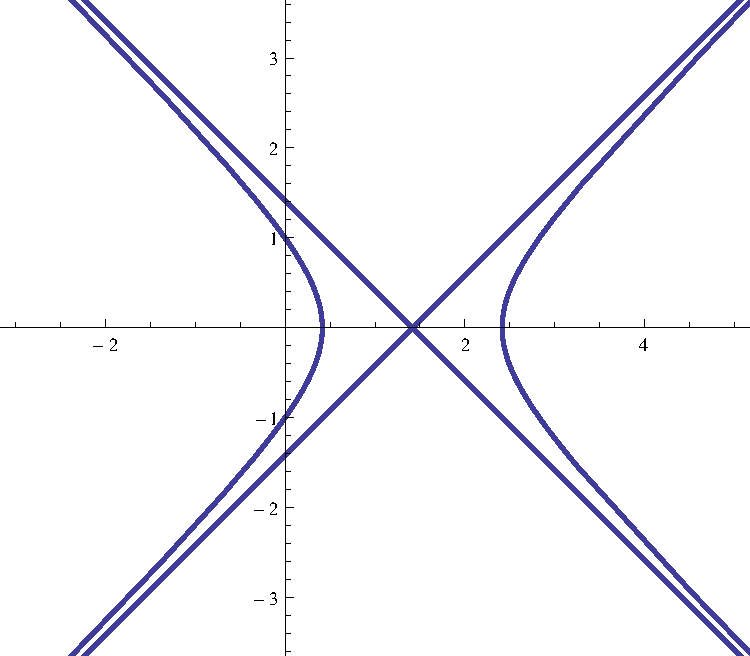
\includegraphics[width=0.35\textwidth]{A14tetel/palyak}
    \caption{A szórócentrum az origóban van. Vonzó kölcsönhatás esetén a bal oldali hiperbola ág mutatja a pályát. Taszító kölcsönhatás esetén a jobb oldali pálya valósul meg. Az ütközési paraméter ($\rho$) a két aszimptota távolsága az origótól.}\label{fig:A14-palyak}
   \end{figure}

   
   Rögzítjük a $q_1$ töltést, $q_2$ töltést pedig szóratjuk a $q_1$ terén. Legyen a töltés taszító, ekkor $\alpha=-k q_1 q_2$. Ekkor a hiperbola megfordul, így az egyenlete:
   \al{
    &r(\varphi)=\frac{-\abs{p}}{1-e\cos(\varphi)}
    &p=\frac{L^2}{m\alpha}=-\frac{m v_\infty^2 \rho^2}{\abs{\alpha}}
    &&e=\sqrt{1+\frac{2EL^2}{m\alpha^2}}
%        =\sqrt{1+\frac{m v_\infty^2 m v_\infty^2 \rho^2}{m\alpha^2}}
       =\sqrt{1+\left(\frac{m  \rho v_\infty^2}{\alpha}\right)^2}.
   }
   
   A két aszimptota a $\varphi_{1,2}=\pm\arccos{\frac{1}{e}}$-nél van, így a szórási szög:
   \al{
    \chi
     &=\pi-(\varphi_1-\varphi_2)
      =\pi-2\arccos\frac{1}{e}
      =2\left(\frac{\pi}{2}-\arccos\frac{1}{e}\right)
      =2\arcsin\frac{1}{e}\\
    \sin\frac{\chi}{2}
     &=\frac{1}{e}
      =\frac{1}{\sqrt{1+\left(\frac{m  \rho v_\infty^2}{\alpha}\right)^2}}\\
     \rho(\chi)
      &=\frac{\abs{\alpha}}{m v_\infty^2}\sqrt{\frac{1}{\sin^2\frac{\chi}{2}}-1}
       =\frac{\abs{\alpha}}{m v_\infty^2}\frac{1}{\tg\frac{\chi}{2}},
   }
   ahonnan a differenciális hatáskeresztmetszet:
   \al{
    \der{\sigma}{\Omega}
     &=\frac{\rho}{\sin\chi}\abs{\der{\rho}{\chi}}
      =\frac{\alpha^2}{m^2 v_\infty^4}\frac{1}{\sin\chi}\frac{1}{\tg\frac{\chi}{2}}\abs{\der{}{\chi}\frac{1}{\tg\frac{\chi}{2}}}
      =\frac{\alpha^2}{m^2 v_\infty^4}\frac{1}{\sin\chi}\frac{1}{\tg\frac{\chi}{2}}\frac{1}{2}\frac{1}{\sin^2\frac{\chi}{2}}\\
     &=\frac{\alpha^2}{m^2 v_\infty^4}\frac{1}{2\sin^2\frac{\chi}{2}}\frac{1}{2}\frac{1}{\sin^2\frac{\chi}{2}}
      =\left(\frac{\alpha}{2m v_\infty^2}\right)^2\frac{1}{\sin^4\frac{\chi}{2}},
   }
   melyből a teljes szórási hatáskeresztmetszet:
   \al{
    \sigma
     &=\intl{}{}\dd\Omega\,\left(\frac{\alpha}{2m v_\infty^2}\right)^2\frac{1}{\sin^4\frac{\chi}{2}}
      =\left(\frac{\alpha}{2m v_\infty^2}\right)^2\intl{0}{\pi}\dd\chi\,2\pi\sin\chi\frac{1}{\sin^4\frac{\chi}{2}}\\
     &=\left(\frac{\alpha}{2m v_\infty^2}\right)^2 4\pi\intl{0}{\pi}\dd\chi\,\frac{\cos\frac{\chi}{2}}{\sin^3\frac{\chi}{2}}
      =\left(\frac{\alpha}{2m v_\infty^2}\right)^2 4\pi\left[-\frac{1}{\sin^2\frac{\chi}{2}}\right]_{0}^{\pi}
      =\text{divergens!}
   }
   
   Ez nem meglepő, a Coulomb-potenciál $\sim\frac{1}{r}$-es, azaz végtelen hatótávolságú. A kísérleti eredményekkel ez ott egyeztethető össze, hogy itt nem vettük figyelembe az árnyékolást, pl. szilárdtestekben való szóródásnál a szóró potenciálra sokkal reálisabb közelítés a $\sim\frac{e^{-r/r_0}}{r}$ alak, aminek hatótávolsága véges, így szórási hatáskeresztmetszete is az.
   
   Megjegyzés: a kvantummechanikai szóráselmélet is a Rutherford-féle formulát adja, a differenciális hatáskeresztmetszetre levezetett összefüggés a kvantummechanikában is helytálló. 
   
 \section{Kvantummechanika}
  
  \subsection{Potenciálszórás}
   
   A kéttest ütközések visszavezethetőek egyrészecske problémára, így a szórásokat úgy vizsgáljuk, hogy egy részecskét szóratunk fix potenciálon. A kísérletileg mérhető differenciális hatáskeresztmetszetet szeretnénk meghatározni a rendszer tulajdonságaiból.
   
   Essen egy monokromatikus $\kv_i$ hullámszámú részecske a szórócentrumra. A potenciál legye rövid hatótávolságú, vagyis $V(\rv)\sim\frac{1}{r^{1+\ep}}$, ahol $\ep>0$. A radiális Schrödinger-egyenlet $r\to\infty$ aszimptotikus megoldása $\mathcal{O}\left(\frac{1}{r}\right)$ rendig:
   \aln{
    \psi(k,\rv)=A\bigg(\underbrace{e^{i\kv_i\rv}}_{\text{be}}+\underbrace{f(\vartheta,\varphi)\frac{e^{i k r}}{r}}_{\text{szórt}}\bigg)
     =\psi_\text{be}(\rv)+\psi_\text{ki}(\rv,k),\label{eq:14-aszimptotikuspsi}
   }
   aminek az első tagja a beeső $\kv_i$ impulzusú síkhullám, a második tagja pedig egy kifutó gömbhullám.
   
   Számoljuk ki a detektoron ($r\to\infty$) a szórási folyamat nélkül beeső hullám, illetve a szórócentrum jelenlétében mérhető részecskeáram-sűrűségének hányadosát. Ebből a deifferenciális haráskeresztmetszet számolható lesz.
   
   A részecskeáram-sűrűség:
   \al{
    \jv(\rv)
     &=\Re\left[\frac{\hbar}{mi}\psi^*(\rv)\grad{\psi(\rv)}\right],
   }
   ahol $\grad=\frac{\partial }{\partial r}\ev_r+\frac{1}{r}\frac{\partial }{\partial \vartheta}\ev_\vartheta+\frac{1}{r \sin\vartheta}\frac{\partial }{\partial \phi}\ev_\varphi\xrightarrow{r\to\infty}\frac{\partial }{\partial r}\ev_r$, így
   \al{
    \jv(\rv)
%      &=\frac{\hbar}{mi}\Re\left[\left(e^{i\kv_i\rv}+f(\vartheta,\varphi)\frac{e^{i\kv\rv}}{r}\right)\frac{\partial }{\partial r}\ev_r\left(e^{i\kv_i\rv}+f(\vartheta,\varphi)\frac{e^{i\kv\rv}}{r}\right)\right],
     &=\Re\left[\frac{\hbar}{mi}\big(\psi^*_\text{be}(\rv)+\psi^*_\text{ki}(\rv,k)\big)\frac{\partial }{\partial r}\ev_r\big(\psi_\text{be}(\rv)+\psi_\text{ki}(\rv,k)\big)\right]\\
     &=\underbrace{\Re\left[\frac{\hbar}{mi}\psi^*_\text{be}(\rv)\grad\psi_\text{be}(\rv)\right]}_{\jv_\text{be}(\rv)}
      +\underbrace{\Re\left[\frac{\hbar}{mi}\psi^*_\text{ki}(\rv,k)\frac{\partial }{\partial r}\psi_\text{ki}(\rv,k)\right]}_{j_\text{sz}(\rv)}\ev_r\\
     &\qquad\qquad+\underbrace{\Re\left[\frac{\hbar}{mi}\left(\psi^*_\text{be}(\rv)\frac{\partial }{\partial r}\psi_\text{ki}(\rv,k)+\psi^*_\text{ki}(\rv,k)\frac{\partial }{\partial r}\psi_\text{be}(\rv)\right)\right]}_{j_\text{interf}(\rv)}\ev_r,
   }
   ahol a $z$ tengely párhuzamos $\kv_i$-vel, így $\kv_i\rv=k_i r\cos\vartheta$. Fejtsük ki a tagokat:
   \al{
    \jv_\text{be}
     &=\Re\left[\frac{\hbar}{mi}A^*\big(e^{-i\kv_i\rv}\big)\grad\big(Ae^{i\kv_i\rv}\big)\right]
      =\Re\left[\frac{\hbar}{mi}\abs{A}^2i\kv_i\right]
      =\abs{A}^2\frac{\hbar\kv_i}{m}
      =\abs{A}^2 \vv_i\\
    \jv_\text{sz}
     &=\Re\left[\frac{\hbar}{mi}\bigg(A^* f^*(\vartheta,\varphi)\frac{e^{-i k r}}{r}\bigg)\frac{\partial }{\partial r}\bigg(A f(\vartheta,\varphi)\frac{e^{i k r}}{r}\bigg)\right]\ev_r\\
     &=\abs{A}^2\Re\left[\frac{\hbar}{mi}\bigg(f^*(\vartheta,\varphi)\frac{e^{-i k r}}{r}\bigg)\bigg(f(\vartheta,\varphi)\partial_r \frac{e^{i k r}}{r}\bigg)\right]\ev_r\\
     &=\abs{A}^2\Re\left[\frac{\hbar}{mi}\bigg(f^*(\vartheta,\varphi)\frac{e^{-i k r}}{r}\bigg)\bigg(f(\vartheta,\varphi)ik\frac{e^{i k r}}{r}\bigg)\right]\ev_r+\mathcal{O}\left(\frac{1}{r^3}\right)\\
     &=\abs{A}^2\abs{f(\vartheta,\varphi)}^2\Re\left[\frac{\hbar}{mi} i k\frac{1}{r^2}\right]+\mathcal{O}\left(\frac{1}{r^3}\right)
      =\abs{A}^2v\ev_r\frac{1}{r^2}\abs{f(\vartheta,\varphi)}^2+\mathcal{O}\left(\frac{1}{r^3}\right)\\
    \jv_\text{interf}
     &=\abs{A}^2\Re\left[\frac{\hbar}{mi}\left(e^{-i\kv_i\rv}\frac{\partial }{\partial r}f(\vartheta,\varphi)\frac{e^{i k r}}{r}+f^*(\vartheta,\varphi)\frac{e^{-i k r}}{r}\frac{\partial }{\partial r}e^{i\kv_i\rv}\right)\right]\ev_r\\
     &=\abs{A}^2\Re\left[\frac{\hbar}{mi}\left(e^{-i\kv_i\rv}f(\vartheta,\varphi)i k\frac{e^{i k r}}{r}+f^*(\vartheta,\varphi)\frac{e^{-i k r}}{r}ik_i\cos\vartheta e^{i\kv_i\rv}\right)\right]\ev_r+\mathcal{O}\left(\frac{1}{r^2}\right).
   }   
   Tegyük fel hogy a szórás rugalmas, azaz $k_i=k$, illetve $v_i=v$, ekkor:
   \al{
    \jv_\text{interf}
     &=\abs{A}^2\frac{1}{r}\Re\left[\frac{\hbar}{mi}\left(ik f(\vartheta,\varphi)e^{i k r(1-\cos\vartheta)}+ikf^*(\vartheta,\varphi)\cos\vartheta e^{-i k r(1-\cos\vartheta)}\right)\right]\ev_r+\mathcal{O}\left(\frac{1}{r^2}\right),
   }
   ami $k$ hulámszámmal oszcillál, amit nem tud a detektor felbontani, így kiátlagolódik. Egyedül akkor nem tűnik el ez a tag, ha $\vartheta=0$.
   
   Innen a differenciális hatáskeresztmetszet \eqaref{eq:14-dhatkm} alapján: $\der{\sigma}{\omega}=\frac{\dd N}{n\dd\Omega}$. Itt $\dd N$ a detektorra érkező részecskeáram és $n$ a forrásból kijövő részecskeáram-sűrűség. Ez a hányados megegyezik a detektorra eső valószínűségi áram $j_\text{sz}A=j_\text{sz}r^2\dd\Omega$ és a bejövő valószínűségi áramsűrűség, vagyis $j_\text{be}$ hányadosával. Behelyettesítve:
   \aln{
    \der{\sigma}{\Omega}
     =\frac{\dd N}{n\dd\Omega}
     =\frac{j_\text{sz}r^2\Omega}{j_\text{be}\dd\Omega}
     =\frac{j_\text{sz}r^2}{j_\text{be}}
     =\frac{\abs{A}^2v\frac{1}{r^2}\abs{f(\vartheta,\varphi)}^2r^2}{\abs{A}^2 v}
     =\abs{f(\vartheta,\varphi)}^2.\label{eq:14-sigma-f}
   }
   
  \subsection{Optikai tétel}
   
   A $\vartheta=0$ esetben az interferencia tag nem hagyható el, az lesz a jelentős. Számítsuk ki egy $\delta\vartheta\to 0$ szögtartományra a részecskeáramot. 
   \al{
    &I_\text{interf}(\delta\vartheta\to 0)\\
    \qquad&=\intl{}{\delta\Omega}\dd\,\Omega r^2 \jv_\text{interf}\ev_r
     =\intl{0}{2\pi}\dd\varphi\intl{0}{\delta\vartheta}\dd\vartheta \sin\vartheta r^2 \jv_\text{interf}\ev_r\\
    \qquad&=\intl{0}{2\pi}\dd\varphi\intl{0}{\delta\vartheta}\dd\vartheta\,\sin\vartheta r^2\abs{A}^2\frac{1}{r}\Re\left[\frac{\hbar}{mi}\left(ik f(\vartheta,\varphi)e^{i k r(1-\cos\vartheta)}+ikf^*(\vartheta,\varphi)\cos\vartheta e^{-i k r(1-\cos\vartheta)}\right)\right]
    \\
    \qquad&\approx-2\pi r\abs{A}^2\Re\left[\frac{\hbar}{mi}\left(ik f(\vartheta=0)\intl{1}{\cos\delta\vartheta}\dd x\,e^{i k r(1-x)}+ikf^*(\vartheta=0)\intl{1}{\cos\delta\vartheta}\dd x\, e^{-i k r(1-x)}\right)\right]
    \\
    \qquad&=-2\pi r\abs{A}^2\Re\left[\frac{\hbar}{m}\left(k f(\vartheta=0)\intl{1}{\cos\delta\vartheta}\dd x\,e^{i k r(1-x)}+\text{komplex konj.}\right)\right]
    \\
    \qquad&=-2\pi r\abs{A}^2\Re\left[\frac{\hbar}{m}\left(k f(\vartheta=0)\left[\underbrace{\frac{e^{i k r(1-\cos{\delta\vartheta})}}{-ikr}}_{\text{oszcillál}\to 0}-\frac{e^{i k r(1-1)}}{-ikr}\right]+\text{komplex konj.}\right)\right]
    \\
    \qquad&\approx-2\pi r\abs{A}^2\Re\left[\frac{\hbar}{m}\left(k f(\vartheta=0)\frac{1}{ikr}+\text{komplex konj.}\right)\right]
    \\
    \qquad&=-2\pi r\abs{A}^2\Re\left[\frac{\hbar}{mi}\left(k f(\vartheta=0)\frac{1}{kr}-\text{komplex konj.}\right)\right]
    \\
    \qquad&=-2\pi r\abs{A}^2\Re\left[2\Im\frac{\hbar}{m}\left[ f(\vartheta=0)\frac{1}{r}\right]\right]
    =-4\pi\abs{A}^2\frac{\hbar}{m}\Im\big[ f(\vartheta=0)\big]
   }
   
   Mivel nem keletkeznek részecskék, ezért a kontinuitási egyenletből következik, hogy
   \al{
    \ointl{\partial V}{}\df\jv(\rv)
     =\ointl{\partial V}{}\df\big(\jv_\text{be}(\rv)+\jv_\text{sz}(\rv)+\jv_\text{interf}(\rv)\big)=0.
   }
   Legyen a térfogat egy szórócentrum körüli $r$ sugarú gömb. A bemenő síkhullám a zárt felületre integrálva nem ad járulékot, az interferencia tag pedig csak $\vartheta=0$ körül:
   \al{
    0
     &=\ointl{\partial V}{}\df\big(\jv_\text{sz}(\rv)+\jv_\text{interf}(\rv)\big)
      =\ointl{\partial V}{}\df\jv_\text{sz}(\rv)+I_\text{interf}(\vartheta\to 0)\\
     &=\ointl{\partial V}{}\df \abs{A}^2v\ev_r\frac{1}{r^2}\abs{f(\vartheta,\varphi)}^2-4\pi\abs{A}^2\frac{\hbar}{m}\Im\big[ f(\vartheta=0)\big]\\
     &=\intl{\partial V}{}\dd\Omega\, \abs{A}^2 v \abs{f(\vartheta,\varphi)}^2-4\pi\abs{A}^2\frac{\hbar}{m}\Im\big[ f(\vartheta=0)\big]
     =\abs{A}^2v\sigma-4\pi\abs{A}^2\frac{\hbar}{m}\Im\big[ f(\vartheta=0)\big],
   }
   ahonnan következik, hogy 
   \al{
    \sigma=4\pi\frac{\hbar}{vm}\Im\big[ f(\vartheta=0)\big]
     =\frac{4\pi}{k}\Im\big[ f(\vartheta=0)\big],
   }
   ez az optikai tétel. Ennek szemléletes jelentése az, hogy a teljes hatáskeresztmetszetet nem csak úgy számolhatom ki, hogy megnézem, hogy mennyi részecske szóródik ki, és azokat összegzem, hanem úgy is, hogy azt nézem meg, hogy hány részecske halad tovább egyenesen.
  
  \subsection{Parciális hullámok módszere}
   
   A Schrödinger-egyenlet (\eqaref{eq:13:radSch} alakjában):
   \al{
     \left[-\frac{\hbar^2}{2m}\frac{1}{r}\partial_r^2r+\frac{\opLv^2}{2mr^2}+V(r)\right]\psi_\kv(r,\vartheta,\varphi)&=E\psi_\kv(r,\vartheta,\varphi),
   }
   ahol a potenciál gömbszimmetrikus, $\kv$ hullámszámmal $z$ irányban érkezik be a hullám, és $E=\frac{\hbar^2 k^2}{2m}$. $m$ itt a redukált tömeget jelenti. Célunk, hogy az egyenlet szórásmegoldásait megkeressük, és azokat összefüggésbe hozzuk \eqaref{eq:14-aszimptotikuspsi} egyenletben felírt alakkal, így az $f(\vartheta)$ függvényt meg tudjuk adni.
   
   Fejtsük ki a megoldást a gömbharmonikusok szerint: 
   \al{
    \psi_k(\rv)=\suml{l=0}{\infty}\suml{m=-l}{l}c_{lm}(k)u_{lm}(k,r)\cdot Y_l^m(\vartheta,\varphi),
   }
   ahol csak az $m=0$ komponens ad járulékot, hiszen a kezdeti feltétel és a probléma is teljesen hengerszimmetrikus. Így $\psi_k(\rv)=\suml{l=0}{\infty}c'_{l}(k)u_{l}(k,r)P_l(\cos\vartheta)$. Innen következik, hogy $f$ is csak $\vartheta$ függvénye lesz az aszimptotikus alakban. A radiális Schrödinger-egyenlet felírva egy $u_l(k,r)$ parciális hullámra:
   \al{
    \left[-\frac{1}{r}\frac{\hbar^2}{2m}\der{^2}{r^2}r+\frac{\hbar^2 l(l+1)}{2mr^2}+V(r)\right]u_l(k,r)&=Eu_l(k,r)=\frac{\hbar^2 k^2}{2m}u_l(k,r),
   }
   ahol $E\Rightarrow k$ folytonos, kontinuum sok $u(k,r)$ megoldással. 
   
   Használjuk ki, hogy nagy távolságra ($r>r_0$) $V(r)\to 0$. Ekkor az egyenlet:
   \al{
    \left[-\frac{1}{r}\frac{\hbar^2}{2m}\der{^2}{r^2}r+\frac{\hbar^2 l(l+1)}{2mr^2}\right]R_l(k,r)&=\frac{\hbar^2 k^2}{2m}R_l(k,r),\\
    \left[\der{^2}{r^2}+\frac{2}{r}\der{}{r}-\frac{l(l+1)}{r^2}+k^2\right]R_l(k,r)&=0\\
    \left[r^2\der{^2}{r^2}+2r\der{}{r}-l(l+1)+k^2r^2\right]R_l(k,r)&=0\\
    \left[(kr)^2\der{^2}{(kr)^2}+2(kr)\der{}{(kr)}-l(l+1)+(kr)^2\right]R_l(kr)&=0,
   }
   ami a gömbi Bessel-féle differenciálegyenlet. Megoldásai a Bessel- ($j_l(kr)$) és a Neumann-függ\-vé\-nyek ($n_l(kr)$). 
   \al{
    &j_l(x) = (-x)^l \frac{1}{x^l}\frac{\dd^l}{\dd x^l}\,\frac{\sin x}{x} ,
    &n_l(x) = -(-x)^l \frac{1}{x^l}\frac{\dd^l}{\dd x^l}\,\frac{\cos x}{x},
   }
   melyek aszimptotikus viselkedése:
   \al{
    &j_l(kr) \xrightarrow{r\to 0} \sim (kr)^l
    &j_l(kr) \xrightarrow{r\to\infty}\frac{1}{kr}\sin\left(kr-\frac{l\pi}{2}\right)\\
    &n_l(kr) \xrightarrow{r\to 0} \sim (kr)^{-l-1}
    &n_l(kr) \xrightarrow{r\to\infty}\frac{1}{kr}\cos\left(kr-\frac{l\pi}{2}\right).
   }
   A $j_l(kr)$ megoldások regulárisak, a $n_l(kr)$-ek pedig irregulárisak. Ezekből a teljes megoldás az $r\to\infty$ határesetben:
   \al{
    u_l(kr)
     \xrightarrow{r\to\infty}&
      C_{l,1}\cdot j_l(kr) +C_{l,2}\cdot n_l(kr)
      =A_l\cos\delta_l\cdot j_l(kr) +A_l\sin\delta_l\cdot n_l(kr)\\
     =&A_l\cos\delta_l\cdot \frac{1}{kr}\sin\left( kr-\frac{l\pi}{2}\right) +A_l\cos\delta_l\cdot \frac{1}{kr}\sin\left(kr-\frac{l\pi}{2}\right)\\
     =&A_l\frac{1}{kr}\sin\left(kr-\frac{l\pi}{2}+\delta_l\right).
   } 
   Ezt behelyettesítve a $\psi_k(r)$ kifejtésbe:
   \al{
    \psi_k(r\to\infty)
     &=\suml{l=0}{\infty}A_l\frac{1}{kr}\sin\left(kr-\frac{l\pi}{2}+\delta_l\right)P_l(\cos\vartheta)\\
     &=\suml{l=0}{\infty}A_l\frac{1}{kr}\frac{1}{2i}\left(e^{ikr}e^{-i\frac{l\pi}{2}+i\delta_l}-e^{-ikr}e^{i\frac{l\pi}{2}-i\delta_l}\right)P_l(\cos\vartheta)\\
     &=\left(\suml{l=0}{\infty}A_l\frac{1}{kr}\frac{1}{2i}e^{-i\frac{l\pi}{2}+i\delta_l}P_l(\cos\vartheta)\right)e^{ikr}
      -\left(\suml{l=0}{\infty}A_l\frac{1}{kr}\frac{1}{2i}e^{i\frac{l\pi}{2}-i\delta_l}P_l(\cos\vartheta)\right)e^{-ikr}.
   }
   Ennek egyenlőnek kell lennie \eqaref{eq:14-aszimptotikuspsi} egyenletben felírt alakkal. Az egyenlőség kifejtéséhez felhasználjuk: $e^{i\kv_i \rv}=e^{ikr\cos\vartheta}=\suml{l=0}{\infty}(2l+1)i^l j_l(kr)P_l(\cos\vartheta)$, így:
   \al{
    \psi(k,\rv)
    &=A\bigg(e^{i\kv_i\rv}+f(\vartheta)\frac{e^{i k r}}{r}\bigg)
     =A\bigg(\suml{l=0}{\infty}(2l+1)i^l j_l(kr)P_l(\cos\vartheta)+f(\vartheta)\frac{e^{i k r}}{r}\bigg)\\
    &\xrightarrow{r\to\infty}A\bigg(\suml{l=0}{\infty}(2l+1)i^l \frac{1}{kr}\sin\left(kr-\frac{l\pi}{2} \right)P_l(\cos\vartheta)+f(\vartheta)\frac{e^{i k r}}{r}\bigg)\\
    &=A\bigg(\suml{l=0}{\infty}(2l+1)i^l \frac{1}{kr}\frac{1}{2i}\left(e^{ikr}e^{-i\frac{l\pi}{2}}-e^{-ikr}e^{i\frac{l\pi}{2}} \right)P_l(\cos\vartheta)+f(\vartheta)\frac{e^{i k r}}{r}\bigg)\\
    &=A\bigg(\suml{l=0}{\infty}(2l+1)i^l \frac{1}{kr}\frac{1}{2i}e^{-i\frac{l\pi}{2}}P_l(\cos\vartheta)+f(\vartheta)\frac{1}{r}\bigg)e^{i k r}\\
    &\qquad\qquad-A\bigg(\suml{l=0}{\infty}(2l+1)i^l \frac{1}{kr}\frac{1}{2i}e^{i\frac{l\pi}{2}} P_l(\cos\vartheta)\bigg)e^{-ikr}.
   }
   Az egyenlőségnek minden $r$-re teljesülni kell, így az exponenciálisok előtti együtthatóknak kell egyenlőnek lenni:
   \al{
    \suml{l=0}{\infty}A_l\frac{1}{kr}\frac{1}{2i}e^{-i\frac{l\pi}{2}+i\delta_l}P_l(\cos\vartheta)
    &=
    A\suml{l=0}{\infty}(2l+1)i^l \frac{1}{kr}\frac{1}{2i}e^{-i\frac{l\pi}{2}}P_l(\cos\vartheta)+Af(\vartheta)\frac{1}{r}
    \\
    \suml{l=0}{\infty}A_l\frac{1}{kr}\frac{1}{2i}e^{i\frac{l\pi}{2}-i\delta_l}P_l(\cos\vartheta)
    &=
    A\suml{l=0}{\infty}(2l+1)i^l \frac{1}{kr}\frac{1}{2i}e^{i\frac{l\pi}{2}} P_l(\cos\vartheta).
   }
   Mivel az egyenletek minden $\vartheta$-ra is igazak, ezért kihasználhatjuk a Legendre-polinomok ortogonalitását is. A második egyenletből $\forall l$-re:
   \al{
    A_l\frac{1}{kr}\frac{1}{2i}e^{i\frac{l\pi}{2}-i\delta_l}
    &=
    A(2l+1)i^l \frac{1}{kr}\frac{1}{2i}e^{i\frac{l\pi}{2}}\\
    \frac{A_l}{A}&=(2l+1)i^l e^{i\delta_l},
   }
   melyet az első egyenletbe helyettesítve:
   \al{
    \suml{l=0}{\infty}(2l+1)i^l e^{i\delta_l}\frac{1}{kr}\frac{1}{2i}e^{-i\frac{l\pi}{2}+i\delta_l}P_l(\cos\vartheta)
    &=
    \suml{l=0}{\infty}(2l+1)i^l \frac{1}{kr}\frac{1}{2i}e^{-i\frac{l\pi}{2}}P_l(\cos\vartheta)+f(\vartheta)\frac{1}{r}
   }
   \al{
    f(\vartheta)
     &=\suml{l=0}{\infty}(2l+1)i^l e^{i\delta_l}\frac{1}{k}\frac{1}{2i}e^{-i\frac{l\pi}{2}+i\delta_l}P_l(\cos\vartheta)-\suml{l=0}{\infty}(2l+1)i^l \frac{1}{k}\frac{1}{2i}e^{-i\frac{l\pi}{2}}P_l(\cos\vartheta)
     \\
     &=\frac{1}{2ik}
       \suml{l=0}{\infty}(2l+1)i^le^{-i\frac{l\pi}{2}}\big(e^{2i\delta_l}-1\big)P_l(\cos\vartheta)
      =\frac{1}{k}
       \suml{l=0}{\infty}(2l+1)i^le^{-i\frac{l\pi}{2}}e^{i\delta_l}\sin(\delta_l) P_l(\cos\vartheta)
      \\
     &=\frac{1}{k}
       \suml{l=0}{\infty}(2l+1)i^l(-i)^l e^{i\delta_l}\sin(\delta_l) P_l(\cos\vartheta)
      =\frac{1}{k}
       \suml{l=0}{\infty}(2l+1) e^{i\delta_l}\sin(\delta_l) P_l(\cos\vartheta).
   }
   Ebből a differenciális hatáskeresztmetszet:
   \aln{
    \der{\sigma}{\Omega}
     &=\abs{f(\theta)}^2
      =\frac{1}{k^2}
       \abs{\suml{l=0}{\infty}(2l+1) e^{i\delta_l}\sin(\delta_l) P_l(\cos\vartheta)}^2.\label{eq:14-diffhatfbol}
   }
   A teljes hatáskeresztmetszethez használjuk az optikai tételt:
   \aln{
    \sigma
     &=\frac{4\pi}{k}\Im\big[ f(\vartheta=0)\big]
      =\frac{4\pi}{k}\Im\left[ \frac{1}{k}\suml{l=0}{\infty}(2l+1) e^{i\delta_l}\sin(\delta_l) \underbrace{P_l(1)}_{=1}\right]\nonumber\\
     &=\frac{4\pi}{k^2}\suml{l=0}{\infty}(2l+1)\sin^2(\delta_l).\label{eq:14-hatfbol}
   }
   
  \subsection{Fázistolás}
   
   Az előzőekben használt $\delta_l$ a fázistolás, mely azt adja meg, hogy a szóródás miatt mekkora fázist szed fel az $l$-edik komponens a szabad megoldáshoz képest. 
   
   Ha a potenciál $r_0$-on kívül nulla, akkor a fázistolások könnyen meghatározhatóak.  Az $r_0$ sugarú gömbön belüli $u_l^{<}(kr)$ és az aszimptotikus $u_l(kr)$ megoldásoknak $r_0$-ban simán kell összeérnie. A simaság itt azt jelenti, hogy az első derivált folytonos $r_0$-ban. Ez akkor folytonos, ha a logaritmus deriváltja is folytonos, így:
   \al{
    \left.\der{}{r}\right|_{r=r_0}\ln u_l(kr)
    =\left.\der{}{r}\right|_{r=r_0}\ln u_l^{<}(kr)
    =\gamma_l(k).
   }
   Itt
   \al{
    \left.\der{}{r}\right|_{r=r_0}\ln u_l(kr)
    &=\left.\der{}{r}\right|_{r=r_0}\ln \big(A_l\cos\delta_l\cdot j_l(kr) +A_l\sin\delta_l\cdot n_l(kr)\big)\\
    &=k\frac{A_l\cos\delta_l\cdot j_l'(kr_0) +A_l\sin\delta_l\cdot n_l'(kr_0)}{A_l\cos\delta_l\cdot j_l(kr_0) +A_l\sin\delta_l\cdot n_l(kr_0)}
     =k\frac{j_l'(kr_0) +\tg\delta_l\cdot n_l'(kr_0)}{ j_l(kr_0) +\tg\delta_l\cdot n_l(kr_0)},
   }
   vagyis 
   \al{
    \tg\delta_l=\frac{k j_l'(kr_0)-\gamma_l(k) j_l(kr_0)}{k n_l'(kr_0)-\gamma_l(k) n_l(kr_0)},
   }
   ahol a $\gamma_l(k)$ a belső térben számolt megoldásból származtatható.
   
  \subsection{A Lippmann--Schwinger-egyenlet, Born-közelítés}
   
   Tekintsük a hullámfüggvény \eqref{eq:14-aszimptotikuspsi} egyenletben kifejtett alakját. A Schrödinger-egyenlet erre felírva:
   \al{
    \left[-\frac{\hbar^2}{2m}\Delta+V(r)\right]\psi_\text{ki}(k,r)&=E\psi_\text{ki}(k,r)=\frac{\hbar^2k^2}{2m}\psi_\text{ki}(k,r)\\
    \left[\Delta+k^2\right]\psi_\text{ki}(k,r)&=\frac{2m}{\hbar^2}V(r)\psi_\text{ki}(k,r).
   }
   Erre tekinthetünk úgy, mint egy inhomogén Laplace-egyenletre, Tudjuk, hogy a Laplace-egyenlet Green-függvénye $G(r-r')=-\frac{1}{4\pi}\frac{e^{ik\abs{r-r'}}}{\abs{r-r'}}$, az inhomogén egyenlet formális megoldása ezzel:
   \al{
    \psi_\text{ki}(k,r)
     =\psi_\text{be}+\frac{2m}{\hbar^2}\intl{}{}\dd r'\, G(r-r')V(r')\psi_\text{ki}(k,r').
   }
   A jobb oldali $\psi_\text{ki}$ helyére beírva az egész kifejezést egy iteratív módszert kapunk $\psi_\text{ki}$ meghatározására. Formálisan felírva a Lippmann--Schwinger-egyenlet: $\psi_\text{ki}=\psi_\text{be}+\opG\opV\psi_\text{ki}$, melynek a megoldása
   \al{
    \psi_\text{ki}
     =\psi_\text{be}+\opG\opV\psi_\text{be}+\opG\opV\opG\opV\psi_\text{be}+\dots
   }
   A Born közelítés, ha csak az elsőrendű járulékot vesszük figyelembe. 
   
 \section{Elektrodinamika -- Kvázistacionárius folyamatok}
  
  \subsection{Kvázistacionárius folyamatok}
   
   Lásd \aref{ss:01-eldidofugges}. és \aref{ss:08-kvazistacdin}. fejezeteket.
   
  \subsection{Indukció}
  
  Kísérleti megfigyelés, hogy zárt áramhurokban elektromotoros erő indukálódik, ha a vezető által körbefogott felületen a mágneses fluxus időben megváltozik. Ez a Faraday-törvény, amelynek matematikai alakja:
  \al{
   \ointl{\partial A}{}\dd\sv\,\Ev(\sv)=-C\der{}{t}\intl{A}{}\df\Bv(\rv),
  }
  ahol $C$ az arányossági tényező. Ennek az arányossági tényezőnek az értékét az rögzíti, hogy az összefüggésnek függetlennek kell lennie a választott koordináta-rendszerről. 
  
  A fluxus megváltozása történhet amiatt, hogy a $\Bv$-nek van időfüggése, illetve amiatt is, hogy a hurok elmozdult. Tekintsünk egy hozzánk képest mozgó hurkot. A szubsztanciális derivált kifejtve:
  \al{
   \der{}{t}\Bv(\rv)
    &=\partial_t\Bv(\rv)+(\vv\cdot\grad)\Bv(\rv),
  }
  ahol felhasználjuk, hogy $\rot(\av\times\bv)=\av(\divo{\bv})-\bv(\divo{\av})+(\bv\divo{})\av-(\av\divo{})\bv$, mellyel
  \al{
   \der{}{t}\Bv(\rv)
    &=\partial_t\Bv(\rv)
      -\rot(\vv\times\Bv(\rv))+\vv(\divo{\Bv(\rv)})-\Bv(\rv)(\divo{\vv})+(\Bv(\rv)\divo{})\vv\\
    &=\partial_t\Bv(\rv)
      -\rot(\vv\times\Bv(\rv)).
  }
  Így
  \al{
   \ointl{\partial A}{}\dd\sv\,\Ev_\text{mozgó}(\sv)
    =-C\der{}{t}\intl{A}{}\df\Bv(\rv)
    =-C\left(\intl{A}{}\df\partial_t\Bv(\rv)-\ointl{\partial A}{}\dd\sv\,\vv\times\Bv(\sv)\right)
  }
  \al{
   \ointl{\partial A}{}\dd\sv\,\big[\Ev_\text{mozgó}(\sv)-C\vv\times\Bv(\sv)\big]
    =-C\intl{A}{}\df\partial_t\Bv(\rv).
  }
  Erre a képletre tekinthetünk másképp is. Tekintsük most a hurkot úgy, hogy az hozzánk képest áll. Akkor ott $\Ev_\text{álló}$ térerősséget mérnék. A Galilei-invariancia alapján $\Ev_\text{álló}=\Ev_\text{mozgó}(\sv)-C\vv\times\Bv(\sv)$, vagyis $\Ev_\text{mozgó}(\sv)=\Ev_\text{álló}(\sv)+C\vv\times\Bv(\sv)$. Ezek azok a térerősségek, melyek a vezetőben hatnak egy töltésre. Az álló rendszerben a töltés nem mozog, ott csak az $\Ev_\text{álló}(\sv)$ hat a töltésre, de ha hozzám képest mozog a vezető, akkor a benne lévő töltések még egy áramot is jelentenek, amire hat a Lorentz-erő. A Lorentz-erővel való összevetésből következik, hogy $C=1$.
  
  \emph{Megjegyzések:} A $C=1$ abból következik, hogy a SI-ben vagyunk. Pl. cgs-ben a Lorenzt-erőben lenne egy $1/c$-s szorzó, akkor $C=1/c$ lenne. Ezen kívül feltűnhet az, hogy az transzformáció elvégzésekor a Galilei-transzformációt hajtottuk végre, és nem a Lorentz-transzformációt. Ez csak a levezetés szempontjából érdekes, azt nem várjuk, hogy az arányossági tényező függjön a sebességtől, így elég az alacsony sebességű  határesetet vizsgálni.
  
  Vezetőhurok nélkül is végigvihető ez a gondolat. Mozgó koordinátarendszerek közötti áttérésnél a Lorentz-transzformáció adja meg a terek transzformációját. Ezek során az elektromos és a mágneses terek is egymásba mennek át (lásd \eqref{eq:A2-Etrafo} és \eqref{eq:A2-Btrafo} egyenletek). Ez éppen azt mondja, hogy az elektromos tér $\vv\times \Bv$-vel változik, ha mozgó rendszerbe térünk át, ami a Lorentz-erőben szereplő megfelelő tagot adja.
  
  Összefoglalva tehát a nyugalmi és a mozgási indukció ugyanaz a jelenség, csak más-más koordinátarendszerből tekintve.
  
  Indukciós együtthatókért lásd \aref{ss:12-indegyh}. fejezetet.
  
  
  \subsection{Örvényáramok}
   
   A kvázisztatikus dinamika alapján a terekre vonatkozó differenciálegyenlet:
   \al{
    \Delta\Hv(t,\rv)=\mu\sigma\partial_t\Hv(t,\rv),
   }
   (lásd \ref{ss:08-kvazistacdin}. fejezet). Oldjuk meg ezt egy félvégtelen anyagra. Legyen a $z>0$ teret kitöltő anyag $\sigma$ a vezetőképességű, $\mu$ a permeabilitású. A $z<0$ tér vákuum. A határon $\Hv=H_0\cos\omega t\cdot \ev_x$ hozunk létre. Kérdés, hogy milyen lesz a mágneses tér. 
   
   A határfeltételek: $\Hv$ véges $z\to\infty$, $z=0$-ban megfelel a peremfeltételnek, és a $\Hv$ tangenciális komponense a felületen változatlanul átmegy. 
   
   Mivel az egyenlet lineáris, ezért a térerősség mindenhol csak $x$ komponenssel rendelkezik, és csak $z$-től és $t$-től függ. A tér időfüggése mindenhol $\sim e^{-i\omega t}$, így az egyenlet:
   \al{
    \partial_z^2 H_x(t,z)&=\mu\sigma\partial_t H_x(t,z)\\
    \partial_z^2 H_x(t,z)&=-i\omega\mu\sigma H_x(t,z)\\
    \left(\partial_z^2+i\omega\mu\sigma \right)H_x(t,z)&=0
   }
   Ez alapján:
   \al{
    &H_x(t,z)=H_0\cdot e^{-i\omega t}e^{ikz}
    &k=\sqrt{i\omega\mu\sigma}=\pm(1+i)\sqrt{\frac{\omega\mu\sigma}{2}}.
   }
   A két $k$ közül azt választjuk ahol $\Im[k]>0$, hogy $z\to\infty$-ben a tér véges legyen, Így tehát a tér levág, a karakterisztikus távolság, azaz a behatolási mélység:
   \al{
    \delta=\sqrt{\frac{2}{\omega\mu\sigma}}.
   }
   Az Ampére-törvény miatt térerősség is indukálódik, amihez áram is tartozik:
   \al{
    &E_y(t,z)=\frac{1}{\sigma}\der{H_z}{z}=\frac{H_0}{\sigma}ik\cdot e^{-i\omega t}e^{ikz}
    &J_y(t,z)
     =\sigma E_y(t,z)
     =H_0ik\cdot e^{-i\omega t}e^{ikz}.
   }
   Az anyagban indukálódott teljes felületi áram:
   \al{
    I_\text{felület,y}
     &=\intl{0}{\infty}\dd z\,J_y(t,z)
      =\intl{0}{\infty}\dd z\,H_0ik\cdot e^{-i\omega t}e^{ikz}
      =H_0\cdot e^{-i\omega t}\big[e^{ikz}\big]_{0}^{\infty}
      =-H_0\cdot e^{-i\omega t},
   } 
   hiszen $\Im[k]>0$. A vezetőben disszipálódott teljesítménysűrűség:
   \al{
    P_\text{ellenállási}
     =\mv{\Jv\Ev}_{t}
     =\mv{\sigma E_y^2}_{t}
     =\mv{\frac{1}{\sigma} H_0^2 k^2\cdot e^{-2i\omega t}e^{i2kz}}_{t}
     =\frac{1}{2} H_0^2\mu\omega e^{-i2z/\delta}.
   }
   
   
   
   
   
